
\section{Training BranchyResNet}

The B-ResNet is trained on the ILSVRC2012 dataset \cite{russakovsky_imagenet_2015}. The model is trained on a single \gls{gpu} GTX1080 with 8Gb memory. Typically a batch size of 32 is chosen, however smaller batch size, have shown better generalization performance \cite{masters_revisiting_nodate}, thus a batch size of 16 is chosen, which also is maximum to prevent memory exhaustion and still have descent training times. The network weights are initialized as pre-trained ImageNet \cite{russakovsky_imagenet_2015}, to reduce model convergence time and improve model accuracy \cite{yosinski_how_2014}. The network classifiers are rough-tuned by freezing the model feature extractor for X epoch with a learning rate of Y. The entire network is then made trainable and trained for Z epochs.

\begin{figure}
	
	\centering
	\captionsetup[subfigure]{justification=centering}
	\subfloat[Train loss\label{fig:B-resnet-voc-train-loss}]{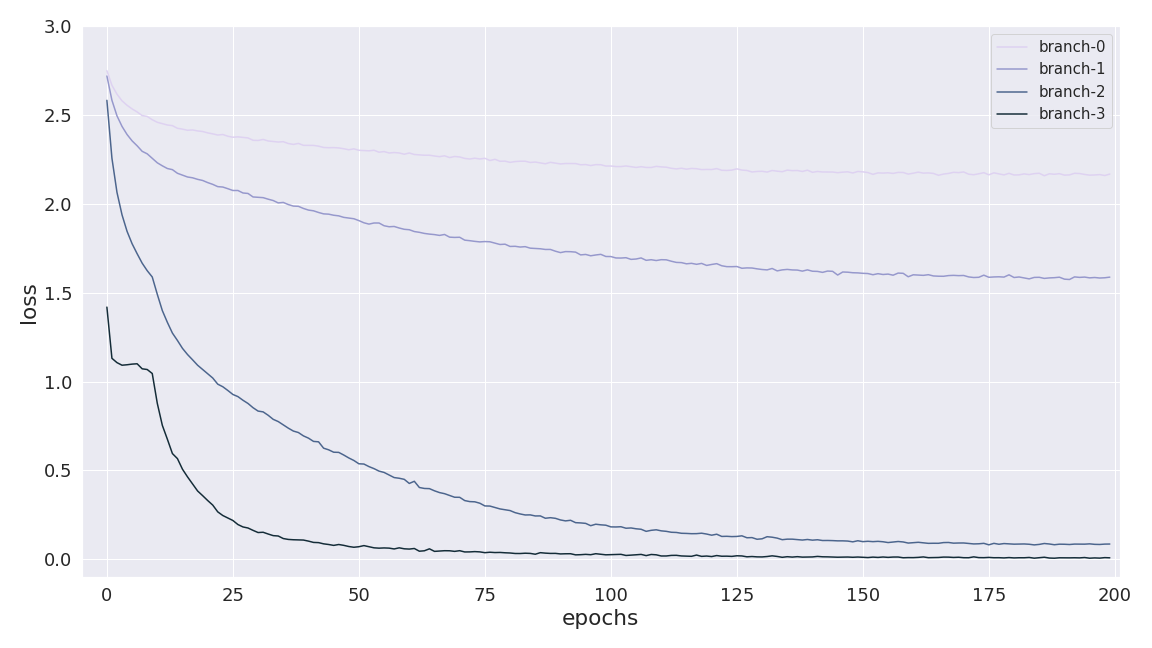
\includegraphics[width=.49\textwidth]{figures/BResNetVOC/BResNet_train_loss_VOC.png}}
	\subfloat[Test loss \label{fig:B-resnet-voc-test-loss}]{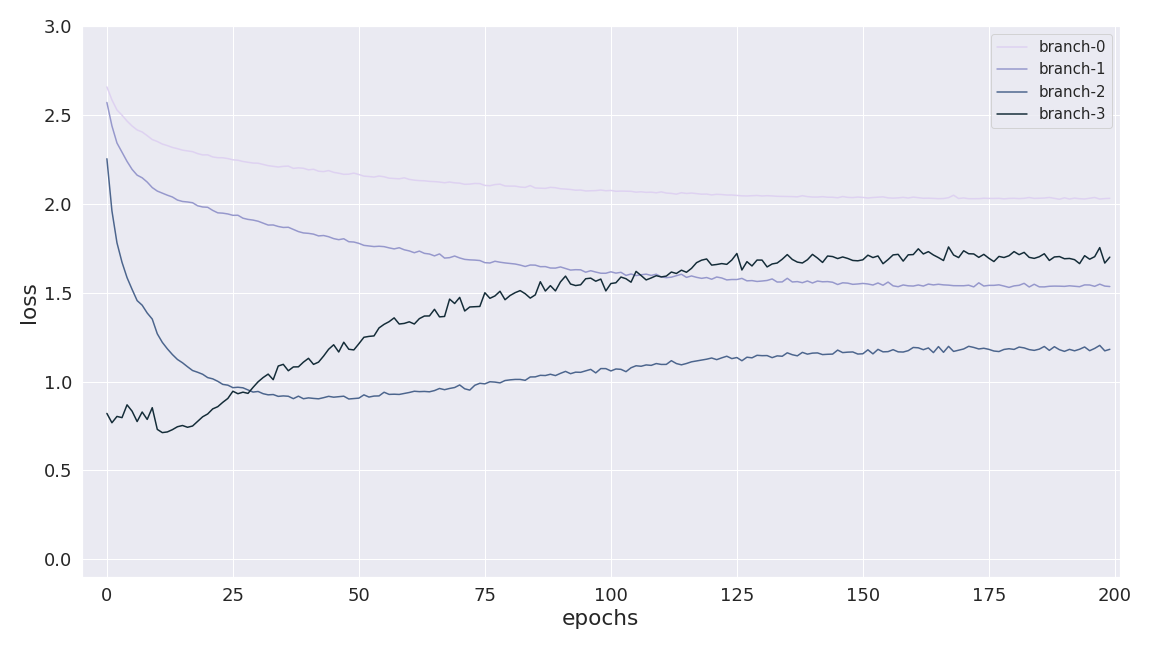
\includegraphics[width=.49\textwidth]{figures/BResNetVOC/BResNet_test_loss_VOC.png}}
	\hfill
	\subfloat[Train accuracy\label{fig:B-resnet-voc-train-acc}]{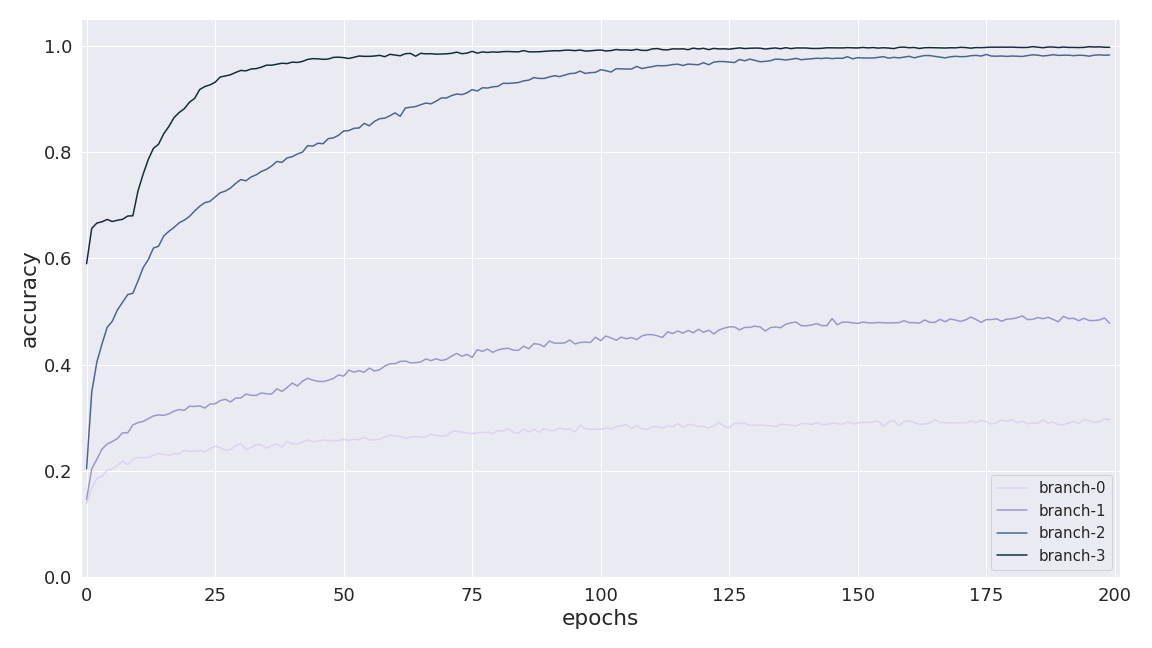
\includegraphics[width=.49\textwidth]{figures/BResNetVOC/BResNet_train_acc_VOC.png}}
	\subfloat[Test accuracy\label{fig:B-resnet-voc-test-acc}]{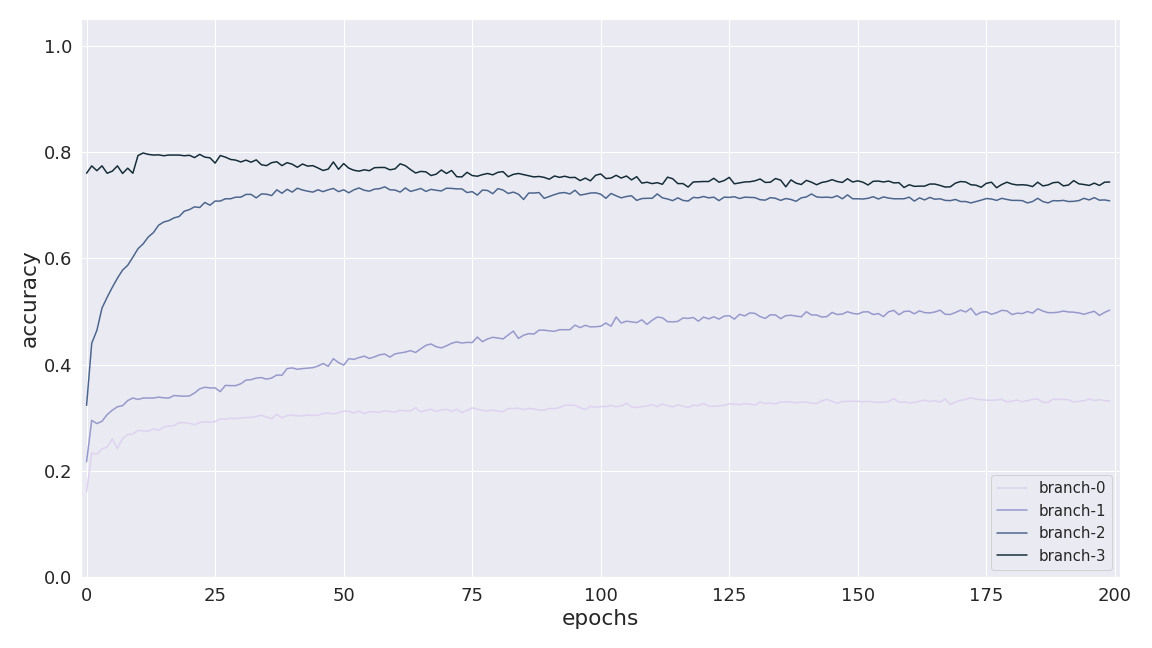
\includegraphics[width=.49\textwidth]{figures/BResNetVOC/BResNet_test_acc_VOC.png}}
	\caption[B-ResNet VOC Training summary]{Training summary shows the progression of model attributes over times of epochs, \protect\subref{fig:B-resnet-voc-train-loss} train loss, \protect\subref{fig:B-resnet-voc-test-loss} test loss, \protect\subref{fig:B-resnet-voc-train-acc} train accuracy, \protect\subref{fig:B-resnet-voc-test-acc}, test accuracy.}
\end{figure}

Visualizing the training progression, clearly indicates that model overfitting to the training data. When a model overfits it suffers to generalize the true underlying distribution of the data. This can be caused by insufficient number of training samples or too complex a model. Since the model has shown promising results in image classification task previously, we can conclude, that the dataset is too sparse.

Even though the model fails to generalize, the experiment still produce interesting results. Given an early exiting model as B-ResNet 50\% of the test samples can be correctly classified using only half of the \gls{dnn}.

\subsection{Optimizer}

The weights of \gls{dnn}s are typically trained using a variant of \gls{sgd}. \gls{sgdr} \cite{loshchilov_sgdr:_2016} is a variant of \gls{sgd}, the method have shown faster convergence on a number of datasets, due to its ability to escape local minimas. It follows a cyclic learning rate schedule in contrast to former decaying learning rate schedules. It has shown, in general, to perform better than adaptive optimizers such as Adam \cite{kingma_adam:_2014}, which also implement strategies to avoid being stuck in local minimas. 

\gls{sgdr} uses an aggressive cosine annealing schedule with warm restarts. Figure \ref{fig:cosineannealing} illustrates the learning rate schedule.

\begin{figure}
	\centering
	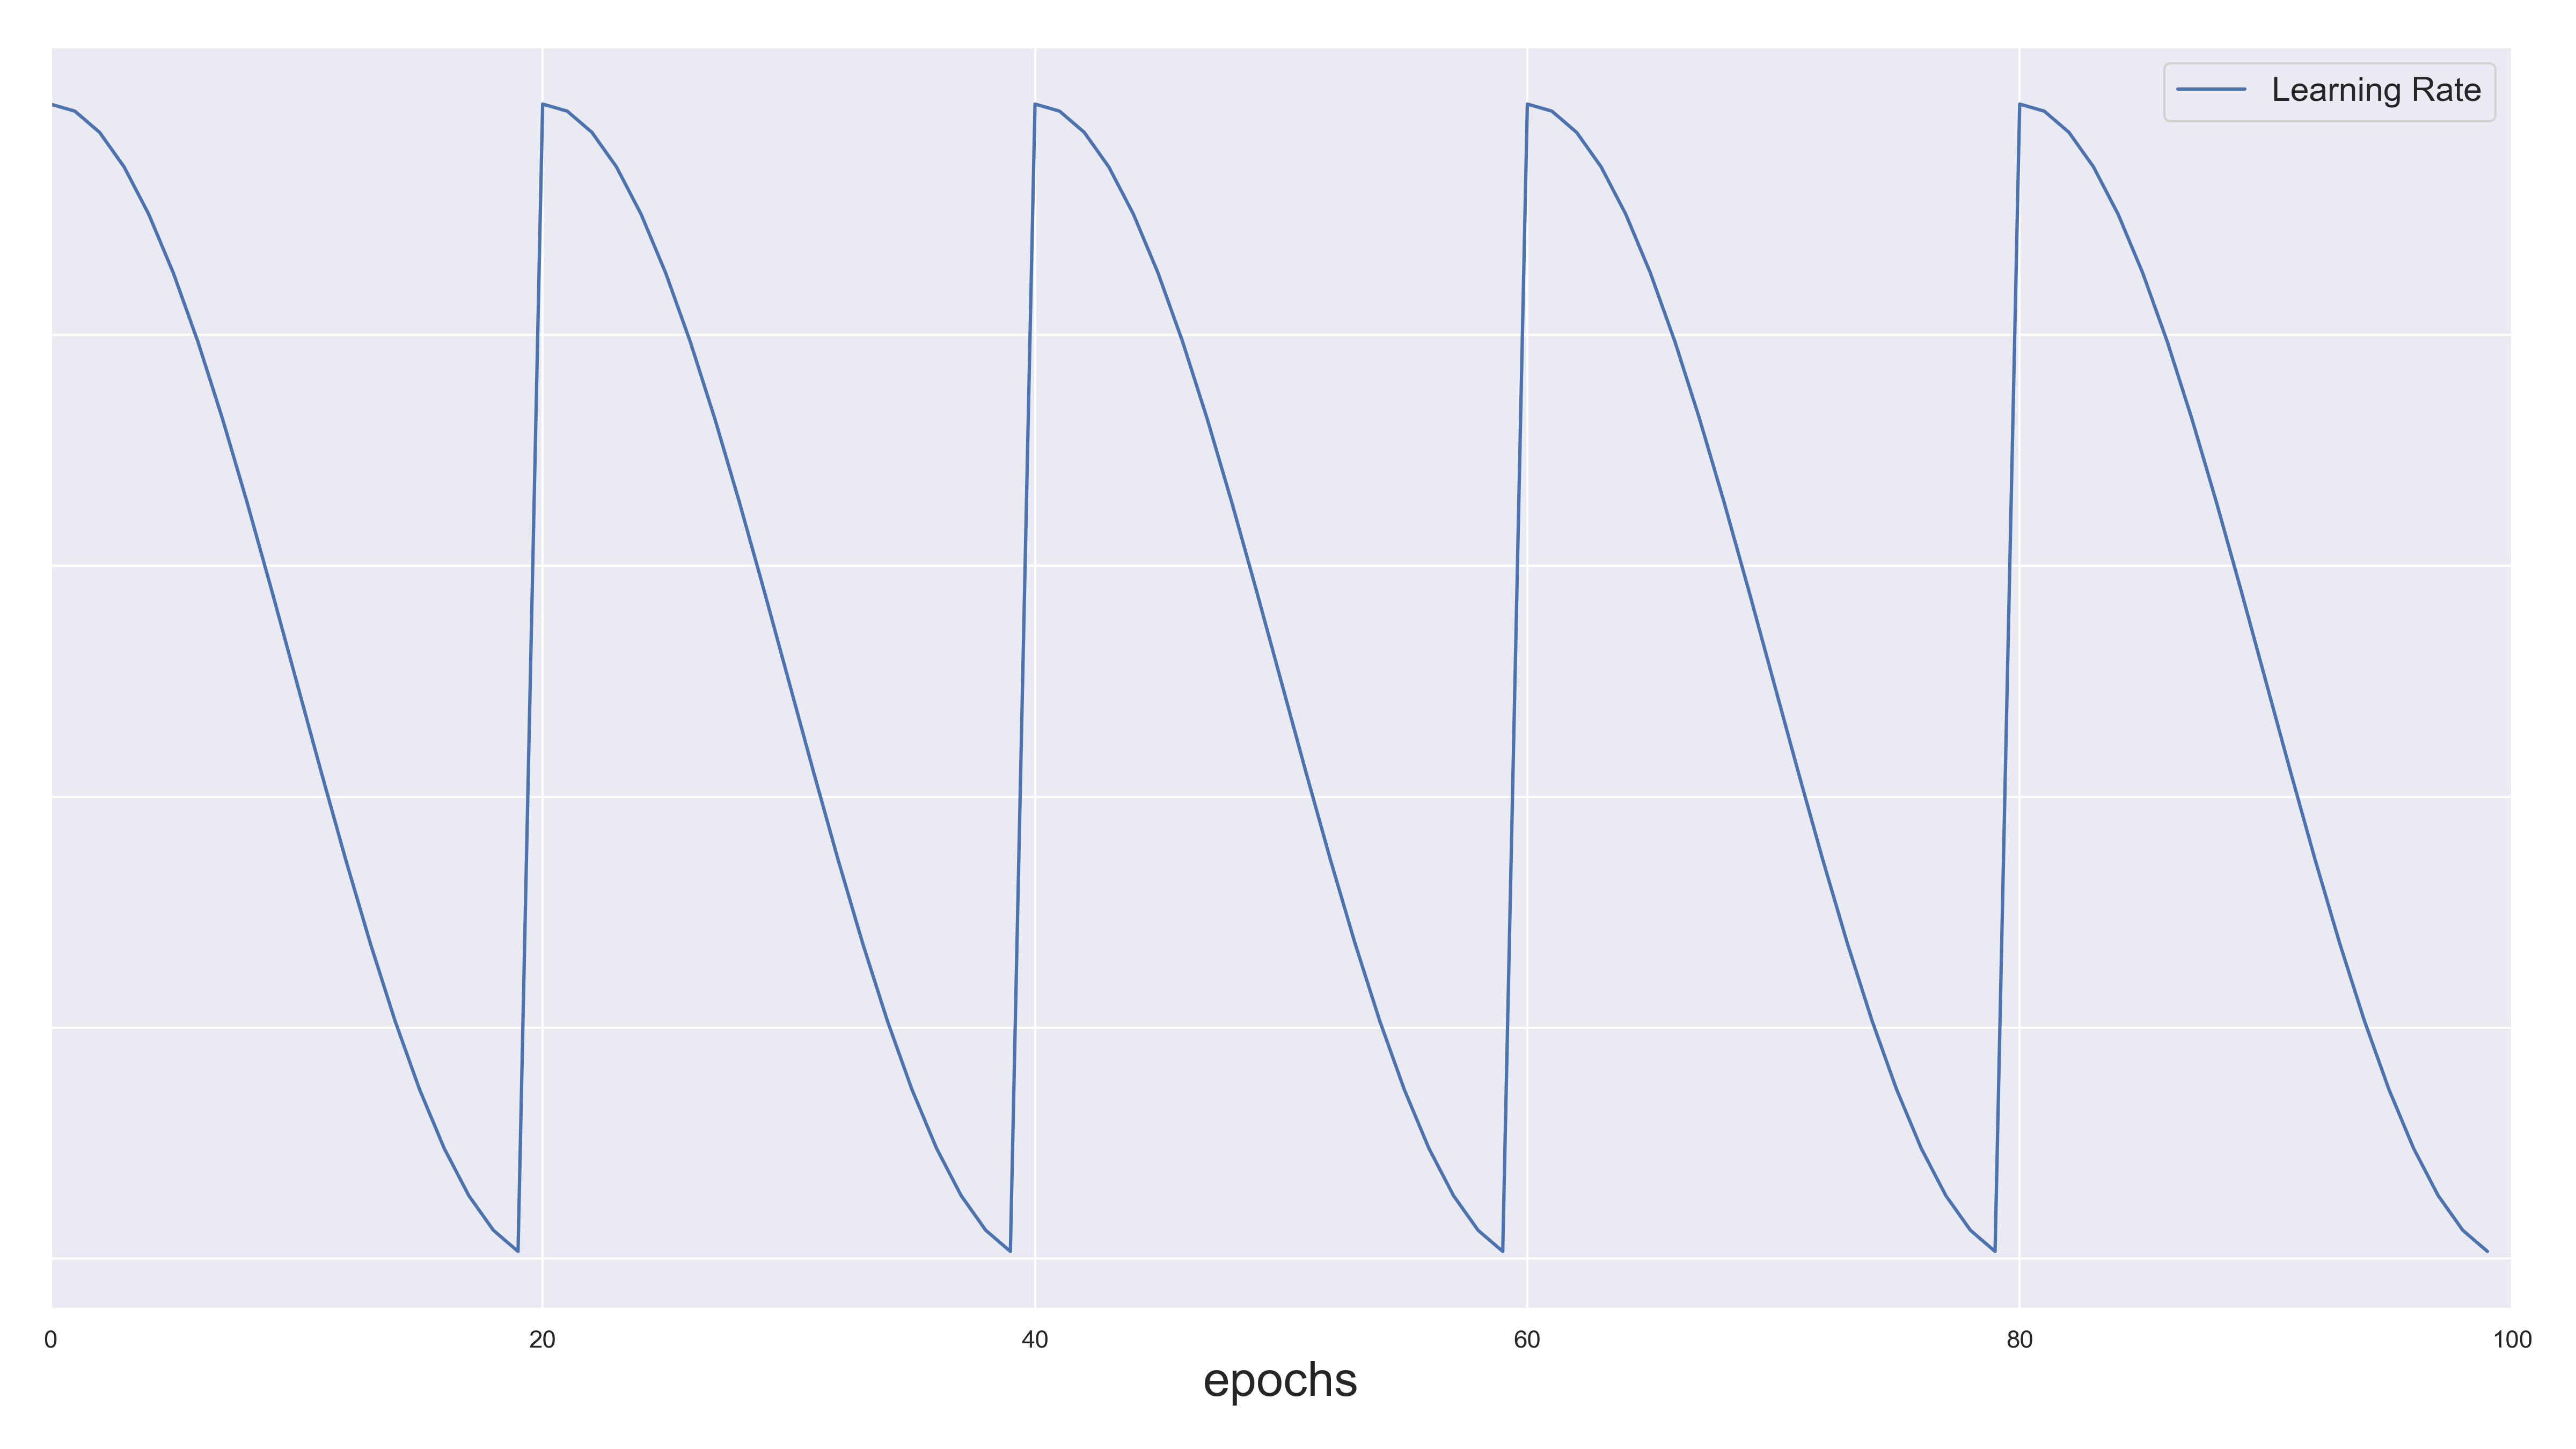
\includegraphics[width=\linewidth]{figures/lr.png}
	\caption[Cosine Annealing Learning Rate]{Cosine Annealing Learning Rate} \label{fig:cosineannealing}
\end{figure}

\subsection{Image Augmentation}

A models ability generalize a specific classification problem has a close connection with the number of available training samples. Data augmentation haven proven to be powerful tool in order to virtually create more training data \cite{perez_effectiveness_2017}. Enlarging a training dataset by data augmentation can help create new versions of an image, that are different from but still similar to the original image, without actually having to acquire and annotate new samples.  

\begin{figure}[H]
	\centering
	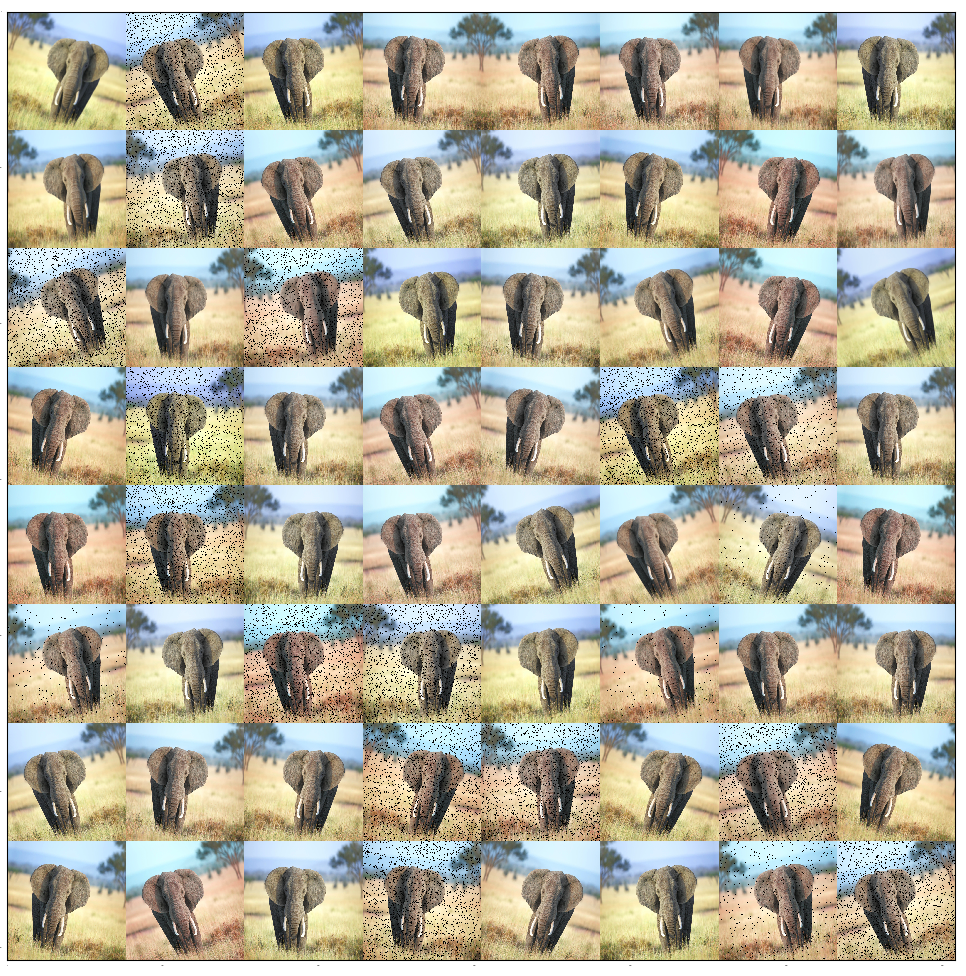
\includegraphics[width=\linewidth]{figures/augmentation/augmentation_high_resolution.png}
	\caption[Image Augmentaion Example]{Image Augmentation of an elephant}
	\label{fig:augmentation}
\end{figure}

Image augmentation involves transformations using tools from image processing to randomly apply noise injection, and color space transformations including contrast and saturation distortions, as well as geometric transformations, such as simple transformations of flipping the image to more complex affine transformations to create different image perspectives \cite{shorten_survey_2019}. Figure \ref{fig:augmentation} shows 64 random augmentations of an image of an elephant. 

New methods have been proposed where image transformations are learned to improve generalization e.g. AutoAugment \cite{cubuk_autoaugment:_2018}. 

Other methods involves actually enlarging the training dataset by synthetically creating more data using a \gls{gan}. \gls{gan}s can help overcome limited data given the available training data or a 3D model, by artificially constructing new samples in different background, light setting and from alternate perspectives.

Methods that do not cover enriching the available training, but alters the learning procedure are called regularization and covers; weight decay, dropout, batch normalization etc. 


\section{Training DDNN}

\section{Transport Protocol} 

Offloading tasks over the network, irregardless fully or partially requires a transport protocol. The selection is typically a choice of either \gls{tcp} or \gls{udp}. \gls{tcp} is a reliable protocol, that guarantee no losses by retransmission of lost packets. \gls{udp} on the other hand is a best-effort protocol, that accept packets loss, thus not introducing retransmission communication overhead. 


Fully offloading \gls{jpeg} compressed images for classification require no losses for human-readability. Sending intermediate features of a \gls{dnn} may not be as intolerant to losses and might be able to function with the far more lightweight \gls{udp}. In current research literature the choice of \gls{tcp} seems given in advance.  

In this experiment the \gls{tcp} transmission time and retransmission rate is investigated under different communication environments. 